% Options for packages loaded elsewhere
\PassOptionsToPackage{unicode}{hyperref}
\PassOptionsToPackage{hyphens}{url}
\PassOptionsToPackage{dvipsnames,svgnames,x11names}{xcolor}
\documentclass[
  10pt,
  fontset=fandol]{ctexart}
\usepackage{xcolor}
\usepackage[margin=16mm]{geometry}
\usepackage{amsmath,amssymb}
\setcounter{secnumdepth}{-\maxdimen} % remove section numbering
\usepackage{iftex}
\ifPDFTeX
  \usepackage[T1]{fontenc}
  \usepackage[utf8]{inputenc}
  \usepackage{textcomp} % provide euro and other symbols
\else % if luatex or xetex
  \usepackage{unicode-math} % this also loads fontspec
  \defaultfontfeatures{Scale=MatchLowercase}
  \defaultfontfeatures[\rmfamily]{Ligatures=TeX,Scale=1}
\fi
\usepackage{lmodern}
\ifPDFTeX\else
  % xetex/luatex font selection
\fi
% Use upquote if available, for straight quotes in verbatim environments
\IfFileExists{upquote.sty}{\usepackage{upquote}}{}
\IfFileExists{microtype.sty}{% use microtype if available
  \usepackage[]{microtype}
  \UseMicrotypeSet[protrusion]{basicmath} % disable protrusion for tt fonts
}{}
\makeatletter
\@ifundefined{KOMAClassName}{% if non-KOMA class
  \IfFileExists{parskip.sty}{%
    \usepackage{parskip}
  }{% else
    \setlength{\parindent}{0pt}
    \setlength{\parskip}{6pt plus 2pt minus 1pt}}
}{% if KOMA class
  \KOMAoptions{parskip=half}}
\makeatother
\usepackage{graphicx}
\makeatletter
\newsavebox\pandoc@box
\newcommand*\pandocbounded[1]{% scales image to fit in text height/width
  \sbox\pandoc@box{#1}%
  \Gscale@div\@tempa{\textheight}{\dimexpr\ht\pandoc@box+\dp\pandoc@box\relax}%
  \Gscale@div\@tempb{\linewidth}{\wd\pandoc@box}%
  \ifdim\@tempb\p@<\@tempa\p@\let\@tempa\@tempb\fi% select the smaller of both
  \ifdim\@tempa\p@<\p@\scalebox{\@tempa}{\usebox\pandoc@box}%
  \else\usebox{\pandoc@box}%
  \fi%
}
% Set default figure placement to htbp
\def\fps@figure{htbp}
\makeatother
\setlength{\emergencystretch}{3em} % prevent overfull lines
\providecommand{\tightlist}{%
  \setlength{\itemsep}{0pt}\setlength{\parskip}{0pt}}
\usepackage{amsmath,amssymb,mathtools,needspace}
\xeCJKDeclareCharClass{CJK}{"2032,"0400->"04FF,"2160->"216B,"2460->"2473,"25A0,"25C7,"25CB,"25CF}
\IfFontExistsTF{Arial Unicode MS}{\xeCJKsetup{AutoFallBack=true}\setCJKfallbackfamilyfont{\CJKrmdefault}{Arial Unicode MS}}{}
\setcounter{secnumdepth}{0}
\setlength{\emergencystretch}{2em}
\allowdisplaybreaks
\usepackage{bookmark}
\IfFileExists{xurl.sty}{\usepackage{xurl}}{} % add URL line breaks if available
\urlstyle{same}
\hypersetup{
  pdftitle={Chebyshev 定理},
  colorlinks=true,
  linkcolor={Maroon},
  filecolor={Maroon},
  citecolor={Blue},
  urlcolor={Blue},
  pdfcreator={LaTeX via pandoc}}

\title{Chebyshev 定理}
\author{}
\date{}

\begin{document}
\maketitle

\subsubsection{3.2.2 Chebyshev 定理}\label{chebyshev-ux5b9aux7406}

这一节要研究最佳逼近多项式的特性, 为此先引进偏差点定义.

定义 3.3 设 \(f(x) \in C[a,b], P(x) \in H_n\), 若在 \(x = x_0\) 上有 \[
|P(x_0) - f(x_0)| = \max_{a \leqslant x \leqslant b}|P(x) - f(x)| = \mu,
\] 则称 \(x_0\) 是 \(P(x)\) 的偏差点.

若 \(P(x_0) - f(x_0) = \mu\), 则称 \(x_0\) 为``正''偏差点.

若 \(P(x_0) - f(x_0) = -\mu\), 则称 \(x_0\) 为``负''偏差点.

由于函数 \(P(x) - f(x)\) 在 \([a,b]\) 上连续, 因此, 至少存在一个点 \(x_0 \in [a,b]\), 使得 \[
|P(x_0) - f(x_0)| = \mu,
\] 也就是说, \(P(x)\) 的偏差点总是存在的. 下面讨论最佳逼近多项式的偏差点性质.

\href{../../source-images/pdf-062.jpeg}{查看原页}

定理 3.3 若 \(P(x) \in H_n\) 是 \(f(x) \in C[a,b]\) 的最佳逼近多项式，则 \(P(x)\) 同时存在正、负偏差点.

证明 因 \(P(x)\) 是 \(f(x)\) 的最佳逼近多项式，故 \(\mu = E_n\). 由于 \(P(x)\) 在 \([a,b]\) 上总有偏差点存在，故可用反证法求证. 不妨假定只有正偏差点，没有负偏差点，于是，对于一切 \(x \in [a,b]\) 都有

\[
P(x) - f(x) > -E_n.
\]

因 \(P(x) - f(x)\) 在 \([a,b]\) 上连续，故有最小值大于 \(-E_n\)，用 \(-E_n + 2h\) 表示，其中 \(h > 0\). 于是，对于一切 \(x \in [a,b]\) 都有

\[
-E_n + 2h \leqslant P(x) - f(x) \leqslant E_n,
\]

\[
-E_n + h \leqslant [P(x) - h] - f(x) \leqslant E_n - h,
\]

即

\[
|[P(x) - h] - f(x)| \leqslant E_n - h.
\]

它表示多项式 \(P(x) - h\) 与 \(f(x)\) 的偏差小于 \(E_n\)，与 \(E_n\) 是最小偏差的假定矛盾.

同样，可证明只有负偏差点没有正偏差点也是不成立的. 证毕.

定理 3.3 的证明从几何上看是十分明显的. 如图 3.2 所示，考察两曲线

\[
y = f(x) + E_n \quad \text{与} \quad y = f(x) - E_n
\]

在 \([a,b]\) 间形成带状区域，曲线 \(y = P(x)\) 在 \([a,b]\) 上就位于这带状区域之间. 定理 3.1 表明，\(P(x)\) 的图形应当与这两条曲线至少各接触一次，这是十分明显的. 若不与 \(y = f(x) - E_n\) 接触，则可把曲线 \(y = P(x)\) 稍向下移动就得到位于曲线 \(y = f(x)\) 较窄带状区域内的曲线 \(y = P(x) - h\). 下面给出反映最佳逼近多项式特征的 Chebyshev 定理.

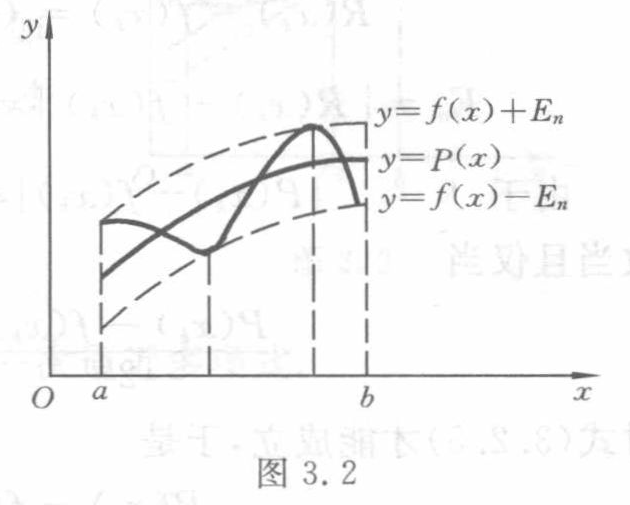
\includegraphics[width=0.85\linewidth,height=\textheight,keepaspectratio,alt={图 3.2 原图裁切}]{../assets/ch03a/fig-3-2.png}

图 3.2（原图）。带状区域及逼近曲线示意；标签为 \(x\)、\(y\)、\(O\)、\(a\)、\(b\)、\(y=f(x)+E_n\)、\(y=P(x)\)、\(y=f(x)-E_n\)。图内还画有从曲线接触点向横轴延伸的竖向辅助线。

定理 3.4 \(P(x) \in H_n\) 是 \(f(x) \in C[a,b]\) 的最佳逼近多项式的充分必要条件是 \(P(x)\) 在 \([a,b]\) 上至少有 \(n+2\) 个轮流为``正''、``负''的偏差点，即有 \(n+2\) 个点 \(a \leqslant x_1 < x_2 < \cdots < x_{n+2} \leqslant b\)，使

\[
\begin{aligned}
P(x_k)-f(x_k)&=(-1)^k\sigma\|P(x)-f(x)\|_\infty,\\
\sigma&=\pm1,\quad k=1,2,\cdots,n+2,
\end{aligned}
\tag{3.2.4}
\]

这样的点组称为 Chebyshev 交错点组.

证明 只证充分性. 假定在 \([a,b]\) 上有 \(n+2\) 个点使式 (3.2.4) 成立，要证明 \(P(x)\) 是 \(f(x)\) 在 \([a,b]\) 上的最佳逼近多项式. 用反证法求证. 若存在 \(Q(x) \in H_n, Q(x) \not\equiv P(x)\)，使

\[
\| f(x) - Q(x) \|_\infty < \| f(x) - P(x) \|_\infty.
\]

由于 \(P(x) - Q(x) = [P(x) - f(x)] - [Q(x) - f(x)]\) 在点 \(x_1, x_2, \cdots, x_{n+2}\) 上的符号与 \(P(x_k) - f(x_k)\) (\(k=1, \cdots, n+2\)) 一致，故 \(P(x) -\)

\begin{quote}
校注（agent 补充，原书疑误）：图 3.2 旁正文印为``定理 3.1 表明''，按原文保留。此段是在解释正、负偏差点同时存在，应指本页定理 3.3；定理 3.1 是 Weierstrass 定理。
\end{quote}

\href{../../source-images/pdf-063.jpeg}{查看原页}

\(Q(x)\) 也在 \(n+2\) 个点上轮流取符号``+''、``-''. 由连续函数性质, 它在 \((a,b)\) 内有 \(n+1\) 个零点, 但 \(P(x)-Q(x) \not\equiv 0\) 是不超过 \(n\) 次的多项式, 它的零点不超过 \(n\). 这个矛盾说明假设不对, 故 \(P(x)\) 就是所求最佳逼近多项式. 充分性得证.

必要性证明较繁, 但证明思想类似定理 3.3, 此处从略.

定理 3.4 说明, 用 \(P(x)\) 逼近 \(f(x)\) 的误差曲线 \(y=P(x)-f(x)\) 是均匀分布的. 由定理 3.4 还可得出以下重要推论.

推论 1 若 \(f(x) \in C[a,b]\), 则在 \(H_n\) 中存在唯一的最佳逼近多项式.

证明 若 \(H_n\) 中有两个最佳逼近多项式 \(P(x)\) 与 \(Q(x)\), 则对于一切 \(x \in [a,b]\), 都有 \[
-E_n \leqslant P(x)-f(x) \leqslant E_n, \quad -E_n \leqslant Q(x)-f(x) \leqslant E_n,
\] 于是 \[
-E_n \leqslant \frac{P(x)+Q(x)}{2}-f(x) \leqslant E_n.
\] 它表明 \(R(x)=\frac{Q(x)+P(x)}{2}\) 也是 \(H_n\) 中的最佳逼近多项式, 因而 \(R(x)-f(x)\) 的 \(n+2\) 个点的交错点组 \(\{x_k\}\) 满足 \[
R(x_k)-f(x_k)=(-1)^k \sigma E_n \quad (k=1,2,\cdots,n+2),
\] \[
E_n=\left|R(x_k)-f(x_k)\right|=\left|\frac{P(x_k)-f(x_k)}{2}+\frac{Q(x_k)-f(x_k)}{2}\right|. \tag{3.2.5}
\] 由于 \(\left|P(x_k)-f(x_k)\right| \leqslant E_n, \quad \left|Q(x_k)-f(x_k)\right| \leqslant E_n\), 故当且仅当 \[
\frac{P(x_k)-f(x_k)}{2}=\frac{Q(x_k)-f(x_k)}{2}=\pm \frac{E_n}{2}
\]

时式 (3.2.5) 才能成立, 于是 \[
P(x_k)-f(x_k)=Q(x_k)-f(x_k).
\] 这就得到 \(P(x_k)=Q(x_k)\) (\(k=1,2,\cdots,n+2\)), 从而表明 \(P(x)-Q(x)\) 有 \(n+2\) 个根. 这个矛盾说明 \(Q(x) \equiv P(x)\), 推论 1 得证.

推论 2 若 \(f(x) \in C[a,b]\), 则其最佳逼近多项式 \(P_n^*(x) \in H_n\) 就是 \(f(x)\) 的一个 Lagrange 插值多项式.

证明 由定理 3.4 可知, \(P_n^*(x)-f(x)\) 在 \([a,b]\) 上要么恒为零, 要么有 \(n+2\) 个轮流取``正''、``负''的偏差点, 于是存在 \(n+1\) 个点 \(x_k \leqslant \overline{x_k} \leqslant x_{k+1}\) (\(k=1,2,\cdots,n+1\)), 使 \(P_n^*(\overline{x_k})-f(\overline{x_k})=0\). 以 \(\overline{x_k}\) 为插值节点的 Lagrange 插值多项式就是 \(P_n^*(x)\).

\subsection{本节覆盖原页的校注记录}\label{ux672cux8282ux8986ux76d6ux539fux9875ux7684ux6821ux6ce8ux8bb0ux5f55}

下列记录按原页关联，含同页相邻小节的校注；计算时同时读取上文校注和完整原页。

\begin{itemize}
\tightlist
\item
  \texttt{ch03a-E02}：原书 PDF 页 62
\end{itemize}

\end{document}
